\chapter{Perancangan}
\label{chap:perancangan}

Pada bab ini akan dibahas mengenai perancangan permainan yang dibangun. Perancangan akan dilakukan meliputi perancangan diagram \textit{sequence}, perancangan diagram kelas, dan perancangan \textit{mockup}.

\section{Diagram Sequence}
Pada bagian ini akan ditunjukan dan dijelaskan diagram sequence Open Source Snake 360. Diagram sequence yang dibuat  meliputi memilih level dan kecepatan. 

\subsection{Memilih Level dan Kecepatan}
\begin{figure}[H]
	\centering  
	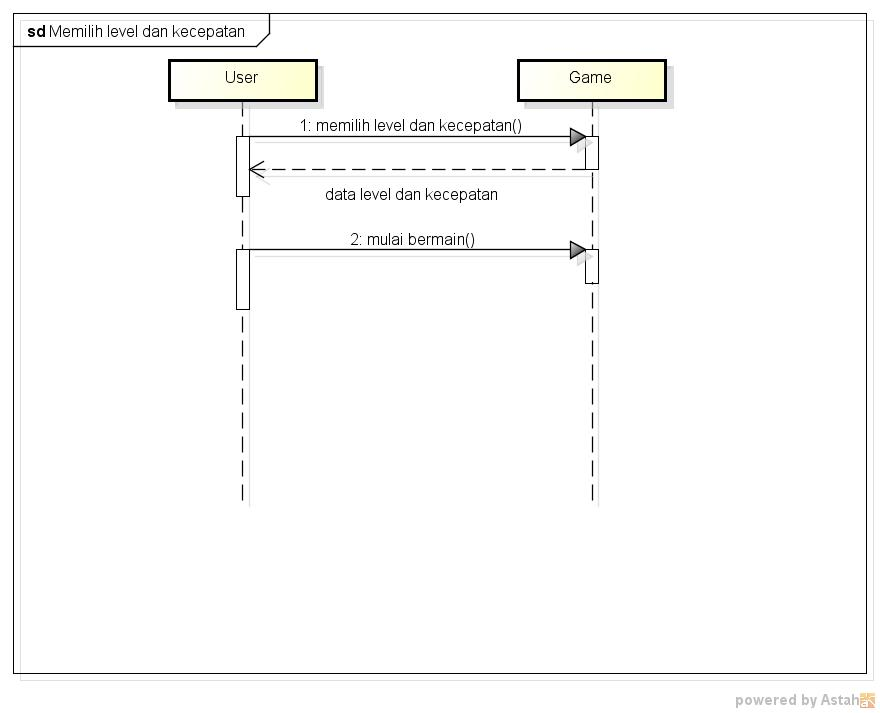
\includegraphics[scale=0.4]{sequencePilih}  
	\caption[Diagram sequence untuk memilih level dan kecepatan]{Diagram sequence untuk memilih level dan kecepatan}
	\label{fig:sequencePilih} 
\end{figure}

Pada Gambar~\ref{fig:sequencePilih}, pemain memulai bermain dengan memilih level dan kecepatan terlebih dahulu. Berikut adalah penjelasan dari Gambar~\ref{fig:sequencePilih}:

\begin{enumerate}
	\item Pemain memilih level labirin dan kecepatan ular. 
	\item Kelas Game akan mengecek apakah input yang dimasukkan oleh user sudah benar atau belum. Jika input belum benar, maka kelas Game akan memberitahu bahwa input yang dimasukkan tidak tepat.
	\item Jika input sudah benar, maka pemain dapat mulai bermain.
\end{enumerate}

\section{Diagram Kelas Rinci}
Pada bagian ini akan ditunjukan dan dijelaskan diagram kelas dari \textit{Open Source Snake 360} secara lengkap. Diagram kelas dapat dilihat pada Gambar~\ref{fig:classDiagramComplete}.

\begin{figure}[H]
	\centering  
	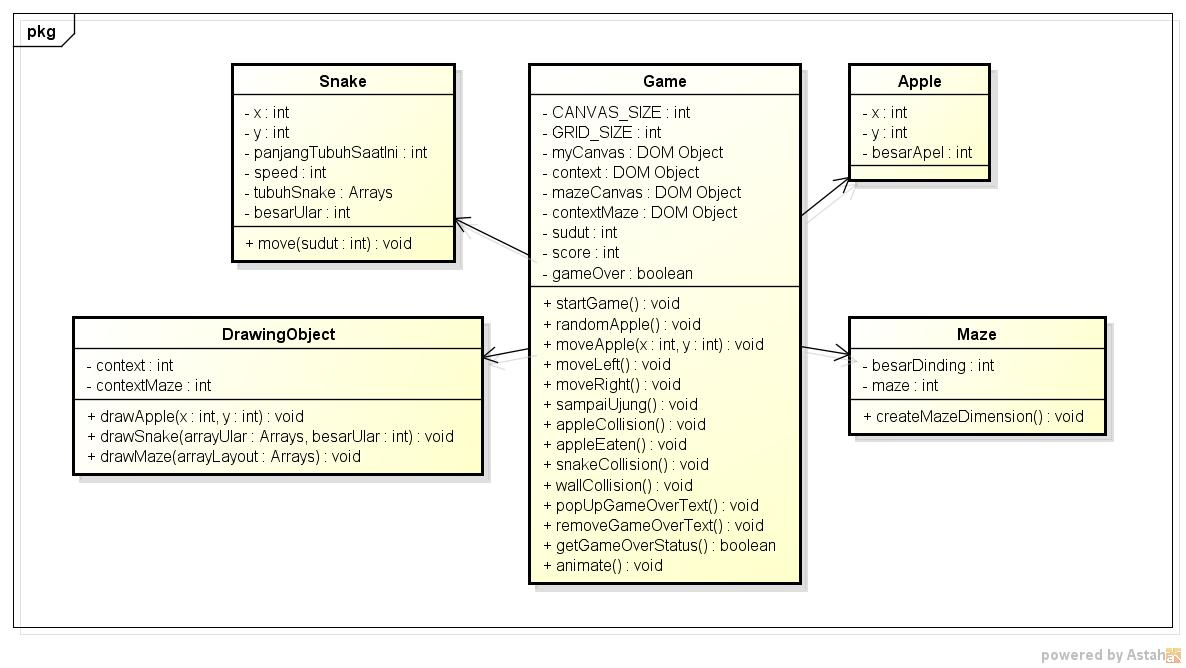
\includegraphics[scale=0.4]{classDiagramComplete}  
	\caption[Diagram class rinci dari Open Source \textit{Snake} 360]{Diagram kelas rinci dari Open Source \textit{Snake} 360}
	\label{fig:classDiagramComplete} 
\end{figure}

\textbf{Deskripsi Kelas dan Method}\\

Pada bagian ini akan dijelaskan deskripsi kelas dan \textit{method-method} pada setiap kelas. Penjelasan kelas dan \textit{method} meliputi nama kelas, deskripsi \textit{method}, input yang dibutuhkan, dan output yang dihasilkan. 

\begin{enumerate}
	\item Kelas \textit{Game} \\
	Kelas \textit{Game} merupakan kelas utama dari permainan ini. Kelas ini mengatur jalannya permainan.
		
		\begin{itemize}
			\item Nama \textit{method} : \textit{startGame}\\
				  Deskripsi : memulai permainan\\
				  Input : tidak ada\\
				  Output : tidak ada\\
			\item Nama \textit{method} : \textit{randomApple}\\
				  Deskripsi : mengacak posisi apel\\
				  Input : tidak ada\\
				  Output : tidak ada\\
			\item Nama \textit{method} : \textit{moveApple}\\
				  Deskripsi : memindahkan posisi apel\\
				  Input : \textit{int} x, \textit{int} y
				  	\begin{itemize}
				  		\item x : koordinat x milik apel
				  		\item y : koordinat y milik apel
				  	\end{itemize}
				  Output : tidak ada\\
			\item Nama \textit{method} : \textit{moveLeft}\\
				  Deskripsi : membuat ular bergerak berlawanan arah jarum jam\\
				  Input : tidak ada\\
				  Output : tidak ada\\
			\item Nama \textit{method} : \textit{moveRight}\\
				  Deskripsi : membuat ular bergerak searah jarum jam\\
				  Input : tidak ada\\
				  Output : tidak ada\\
			\item Nama \textit{method} : sampaiUjung\\
				  Deskripsi : membuat ular akan muncul di sisi yang berlawanan ketika ular sudah mencapai ujung labirin\\
				  Input : tidak ada\\
				  Output : tidak ada\\
			\item Nama \textit{method} : \textit{appleColiision}\\
				  Deskripsi : mengecek tabrakan antara apel dengan kepala ular\\
				  Input : tidak ada\\
				  Output : tidak ada\\
			\item Nama \textit{method} : \textit{appleEaten}\\
				  Deskripsi : aksi yang dilakukan apabila ular sudah memakan apel\\
				  Input : tidak ada\\
				  Output : tidak ada\\
			\item Nama \textit{method} : \textit{snakeCollision}\\
				  Deskripsi : mengecek tabrakan antara kepala ular dengan tubuhnya sendiri\\
				  Input : tidak ada\\
				  Output : tidak ada\\
			\item Nama \textit{method} : \textit{wallCollision}\\
				  Deskripsi : mengecek tabrakan antara kepala ular dengan dinding labirin\\
				  Input : tidak ada\\
				  Output : tidak ada\\
			\item Nama \textit{method} : \textit{popUpGameOverText}\\
				  Deskripsi : memunculkan tulisan 'Game Over'\\
				  Input : tidak ada\\
				  Output : tidak ada\\
			\item Nama \textit{method} : \textit{removeGameOverText}\\
				  Deskripsi : menghilangkan tulisan 'Game Over'\\
				  Input : tidak ada\\
				  Output : tidak ada\\
			\item Nama \textit{method} : \textit{getGameOverStatus}\\
				  Deskripsi : mendapatkan status gameOver\\
				  Input : tidak ada\\
				  Output : \textit{boolean gameOver}
				  	\begin{itemize}
				  		\item \textit{gameOver} : status apapbila permainan sudah berakhir atau belum
				  	\end{itemize}
			\item Nama \textit{method} : \textit{animate}\\
				  Deskripsi : membuat animasi dari setiap objek\\
				  Input : tidak ada\\
				  Output : tidak ada
		\end{itemize}
		
	\item Kelas \textit{Snake}\\
	Kelas \textit{Snake} merupakan kelas yang merepresentasikan objek ular.
		
		\begin{itemize}
			\item Nama \textit{method} : \textit{move}\\
				  Deskripsi : memulai permainan\\
				  Input : \textit{int} x, \textit{int} y
				  	\begin{itemize}
				  		\item x : koordinat x milik ular
				  		\item y : koordinat y milik ular
				  	\end{itemize}
				  Output : tidak ada\\
		\end{itemize}
		
	\item Kelas \textit{DrawingObject}\\
	Kelas \textit{DrawingObject} merupakan kelas yang bertugas untuk menggambar objek-objek yang terdapat pada canvas.
	
		\begin{itemize}
			\item Nama \textit{method} : \textit{drawApple}\\
				  Deskripsi : menggambar objek apel\\
				  Input : int x, int y
				  	\begin{itemize}
				  		\item x : koordinat x milik apel
				  		\item y : koordinat y milik apel
				  	\end{itemize}
				  Output : tidak ada\\
			\item Nama \textit{method} : \textit{drawSnake}\\
				  Deskripsi : menggambar objek ular\\
				  Input : \textit{int}[] arrayUlar, \textit{int} besarUlar
				  	\begin{itemize}
				  		\item arrayUlar : koordinat x dan y milik setiap bagian tubuh ular
				  		\item besarUlar : lebar tubuh ular
				  	\end{itemize}
				  Output : tidak ada\\
			\item Nama \textit{method} : \textit{drawMaze}\\
				  Deskripsi : menggambar labirin\\
				  Input : \textit{String arrayLayout}, \textit{int besarDinding}
				  	\begin{itemize}
				  		\item \textit{arrayLayout} : layout labirin yang akan digambar
				  		\item besarDinding : besar dinding labirin
				  	\end{itemize}
				  Output : tidak ada\\
		\end{itemize}
		
\end{enumerate} 

\section{Mockup}
Pada bagian ini akan ditunjukan rancangan antarmuka dari permainan yang dibangun yang terdiri dari menu pemilihan level, mulai bermain, dan permainan berakhir.

\subsection{Tampilan Menu Utama}
Gambar~\ref{fig:menuUtama} merupakan rancangan tampilan awal dari permainan yang dibangun. Pada tampilan ini terdapat judul permainan, 2 buah input untuk memilih level dan kecepatan gerak ular, dan tombol OK. Tampilan menu utama akan menampilkan pesan kesalahan seperti terdapat pada Gambar~\ref{fig:menuUtamaSalah}. Apabila pemain salah memasukkan data, maka permainan tidak akan dimulai jika tombol OK ditekan.

\begin{figure}[H]
	\centering  
	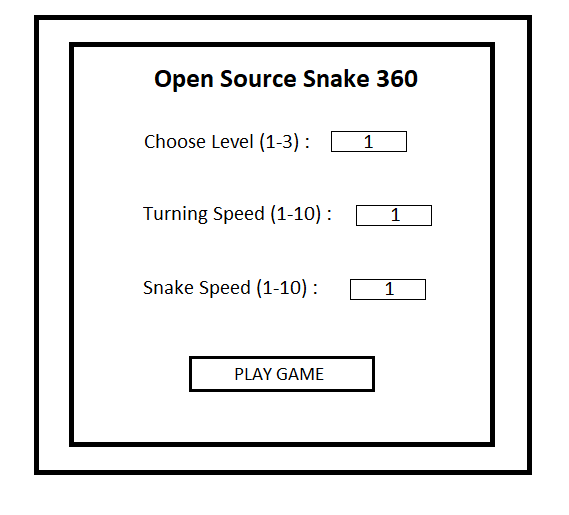
\includegraphics[scale=0.5]{menuUtama}  
	\caption[Rancangan tampilan menu utama]{Rancangan tampilan menu utama}
	\label{fig:menuUtama} 
\end{figure}

\begin{figure}[H]
	\centering  
	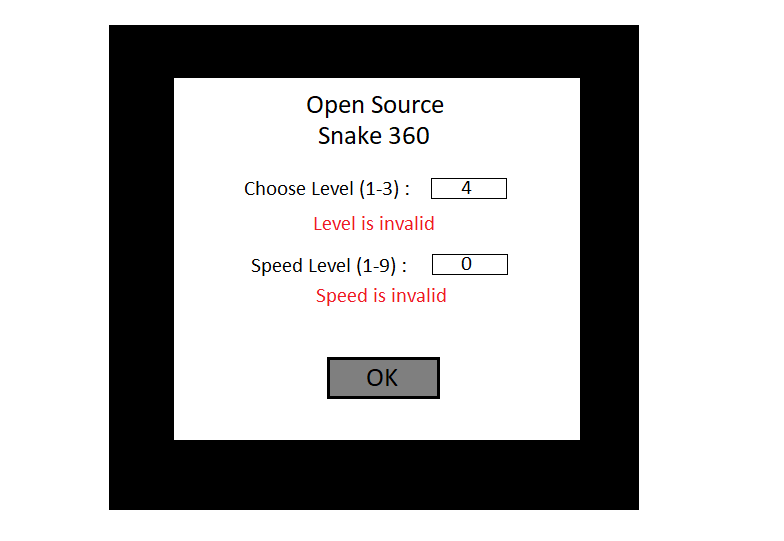
\includegraphics[scale=0.5]{menuUtamaSalah}  
	\caption[Rancangan tampilan menu utama jika pemain salah memasukkan data]{Rancangan tampilan menu utama jika pemain salah memasukkan data}
	\label{fig:menuUtamaSalah} 
\end{figure}

\subsection{Tampilan Bermain}
Tampilan bermain akan muncul setelah pemain memilih level dan kecepatan ular pada menu utama dengan benar dan menekan tombol OK (Gambar~\ref{fig:menuUtama}). Gambar~\ref{fig:permainan} merupakan tampilan permainan sudah dimulai. Pada tampilan ini terdapat ular, dinding labirin dan makanan berbentuk apel. Pada tampilan ini juga terdapat level labirin yang dipilih dan skor yang didapat. 

\begin{figure}[H]
	\centering  
	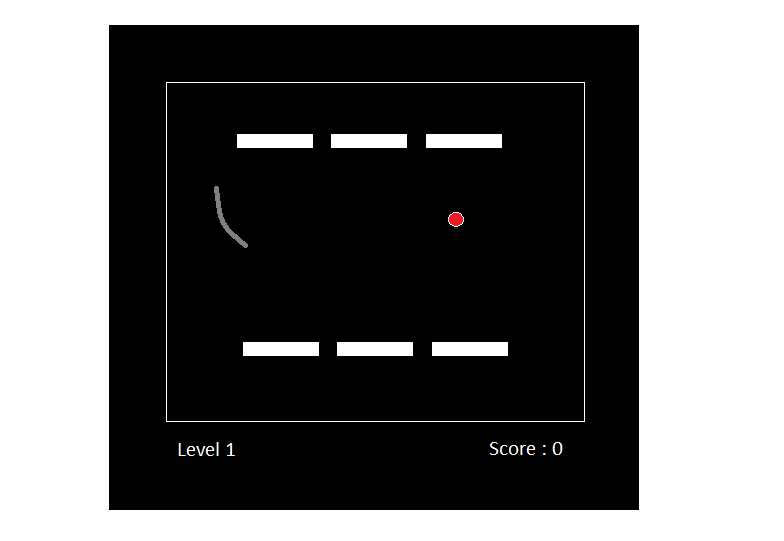
\includegraphics[scale=0.5]{permainan}  
	\caption[Rancangan tampilan bermain]{Rancangan tampilan bermain}
	\label{fig:permainan} 
\end{figure}

\subsection{Tampilan Permainan Berakhir}
Tampilan ini akan muncul apabila permainan berakhir. Permainan akan berkahir jika ular menabrak dinding labirin atau menabrak tubuhnya sendiri. Gambar~\ref{fig:permainanBerakhir} merupakan tampilan permainan berakhir. Pada tampilan ini, pemain dapat mengulang permainan dengan menekan tombol 'ENTER'. Pemain akan dialihkan ke tampilan menu utama(Gambar~\ref{fig:menuUtama}) apabila tombol 'ENTER' ditekan.


\begin{figure}[H]
	\centering  
	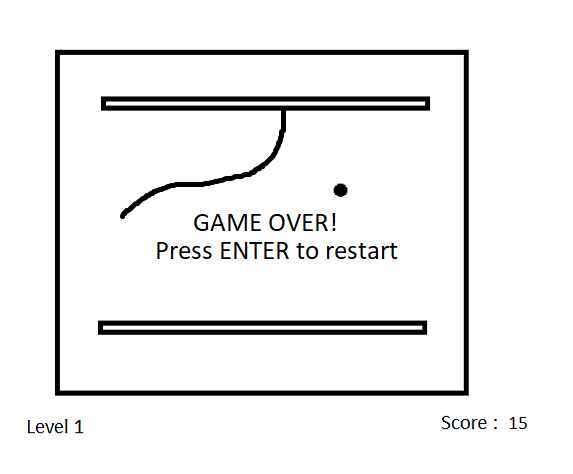
\includegraphics[scale=0.5]{permainanBerakhir}  
	\caption[Rancangan tampilan permainan berakhir]{Rancangan tampilan permainan berakhir}
	\label{fig:permainanBerakhir} 
\end{figure}